\documentclass[a0]{a0poster}

\usepackage[paperheight=30in, paperwidth=42in, margin=1.5in]{geometry}

\usepackage{tgpagella}

\usepackage{multicol}
\usepackage{amsmath}
\usepackage{bm}
\usepackage{titlesec}
\usepackage{graphicx} % Required for including images
\usepackage[backend=bibtex]{biblatex}
\usepackage{tikz}
\usepackage{relsize}

% Required for specifying captions to tables and figures
\usepackage{amsfonts, amsmath, amsthm, amssymb}
\usepackage[most]{tcolorbox}

\newcommand{\eqskip}{20pt}
\setlength{\abovedisplayskip}{\eqskip}
\setlength{\belowdisplayskip}{\eqskip}
\setlength{\abovedisplayshortskip}{\eqskip}
\setlength{\belowdisplayshortskip}{\eqskip}

\usetikzlibrary{arrows,arrows.meta,automata}
\bibliography{poster}

\def\bibfont{\Large}

% Math shorthands
\newcommand{\paren}[1]{\left(#1\right)}
\newcommand{\Z}{\mathbb Z}
\newcommand{\N}{\mathbb N}
\newcommand{\Q}{\mathbb Q}
\newcommand{\A}{\mathcal A}
\newcommand{\F}{\mathcal F}
\newcommand{\M}{\mathcal M}
\newcommand{\bin}{\pmb{\bm{2}}}
\newcommand{\sg}[1]{\mathcal S\paren{#1}}
\newcommand{\gp}[1]{\mathcal G\paren{#1}}
\newcommand{\orb}{\mathbf{orb}}
\newcommand{\aut}[1]{\underline{#1}}
\renewcommand{\d}[1]{\partial_{#1}\,}
\newcommand{\floor}[1]{\left\lfloor#1\right\rfloor}
\newcommand{\ffrac}[2]{\floor{\frac{#1}{#2}}}
\newcommand{\ceil}[1]{\left\lceil#1\right\rceil}
\renewcommand{\cfrac}[2]{\ceil{\frac{#1}{#2}}}
\newcommand{\vecc}{\textbf{vec}}
\newcommand{\nll}{\textbf{null}}


%\definecolor{CMUMaroon}{RGB}{128,6,6}
\definecolor{CMUMaroon}{RGB}{118,6,6}
\newtcolorbox{poster-header}[1][]
{
    colframe = CMUMaroon,
    colback  = CMUMaroon,
    boxrule  = 5mm,
    boxsep   = 5mm,
    #1,
}

\newtcolorbox{poster-section}[2][]
{
    colframe = CMUMaroon,
    boxrule  = 3mm,
    boxsep   = 3mm,
    coltitle = white,
    boxsep = 8mm,
    title    = \centering\Huge#2,
    #1,
}

\begin{document}

\begin{poster-header}
    \begin{center}
        \color{white}
        \veryHuge
        {\bf{Orbit Rational Transducers}}\\
        \huge {Tim Becker \& Klaus Sutner}
    \end{center}
\end{poster-header}

\columnsep=50pt
\begin{multicols}{2}

\begin{poster-section}{Abstract}
    \Large
    We study the complexity arising from iterating transductions in invertible
    transducers and give an algorithm to decide if an abelian transducer has
    rational orbit relations. The algorithm leverages a connection between
    abelian automaton groups and algebraic number fields.
\end{poster-section}

\begin{poster-section}{Invertible Transducers}
\Large
We are interested in transducers over the binary alphabet $\bin$ whose
transductions are invertible --- the output function for each state is a
permutation of $\bin$. A state is called \emph{odd} if its output function is
the transposition and \emph{even} otherwise.
\begin{center}
    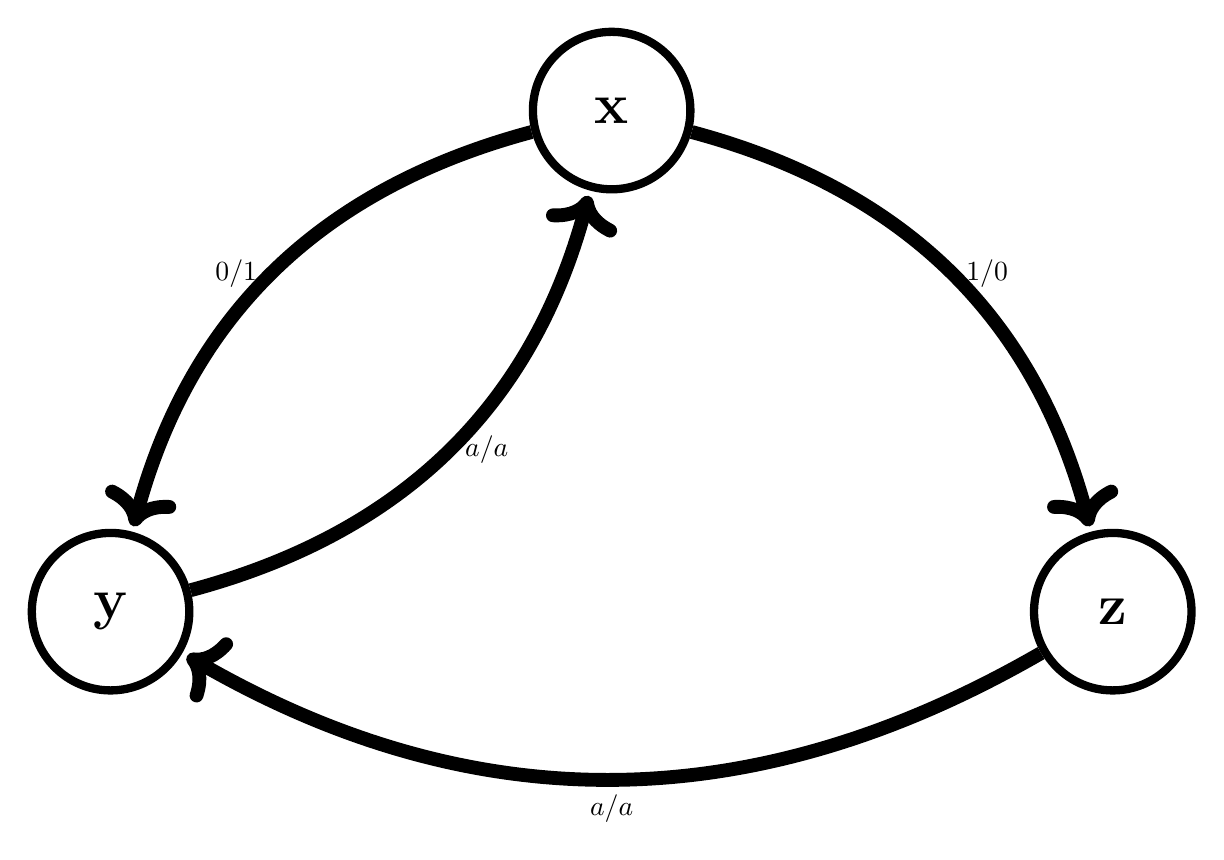
\begin{tikzpicture}[
        ->,
        auto,
        shorten > = 2pt, % don't touch arrow head to node
        node distance=9cm]

        \tikzstyle{every state}=[
            draw = black,
            style = thick,
            fill = white,
            line width = 3pt,
            minimum size = 20mm
        ]
        \tikzstyle{every edge}=[
            style = thick,
            draw = black,
            line width=5pt,
        ]
        \tikzset{l/.style={font=\huge}}
        \node[l,state] (0) {$\mathbf{x}$};
        \node[l,state] (1) [below left of =0] {$\mathbf{y}$};
        \node[l,state] (2) [below right of =0] {$\mathbf{z}$};
        \path
        (0) edge[bend right, left]
        node {$0/1$} (1)
        (0) edge[bend left, right]
        node {$1/0$} (2)
        (1) edge[bend right, right]
        node {$a/a$} (0)
        (2) edge[bend left]
        node {$a/a$} (1)
        ;
    \end{tikzpicture}
\end{center}
The transductions of such a machine are length-preserving bijections on
$\bin^*$. These transductions form a semigroup under composition.
When they commute with one another, we call the transducer \emph{abelian}.\\

The \emph{residuals} of a transduction $f$, denoted $f_0$ and $f_1$, are the
induced transductions after reading one character. In the above example
$\mathbf{x}_0 = \mathbf{y}$ and $\mathbf{z}_0 = \mathbf{z}_1 = \mathbf{y}$.
\end{poster-section}
\begin{poster-section}{Orbit Relation}
\Large
The \emph{orbit relation} of a transduction $f$ is defined as
\[
    \orb(f) = \{(x,y) \mid \exists t \in \N \,.\, f^t(x) = y\}
\]
Because $f$ is a length-preserving bijection on $\bin^*$,
$\orb(f)$ is an equivalence relation.
\end{poster-section}

\begin{poster-section}{Orbit Rationality}
    \Large
    We studied the complexity of deciding the orbit relation and found that
    in some cases, the relation is \emph{rational}, meaning it can be decided
    by a finite state machine.\\\\
    \textbf{Theorem:}
    One can efficiently decide if an abelian transducer is orbit-rational.\\

    \textbf{Proof Sketch:}
    We will work in the semigroup of transductions. Then, $\orb(f)$ being
    rational is equivalent to the finiteness of the transitive closure of the
    following map applied to $f$
    \[
        \varphi(f) = \begin{cases}
            f_0 &\text{if $f$ is even}\\
            (f^2)_0 &\text{if $f$ is odd}
        \end{cases}
    \]
    To each abelian transducer, we can associate (and efficiently compute) an
    algebraic number field $\F = \Q(\alpha)$ and view the semigroup as elements
    of $\F$.\\

    Residuation in the semigroup corresponds to an affine map in $\F$: the
    transition $p \xrightarrow{a / b} q$ in the transducer corresponds to
    $\alpha p + (b - a) = q$ in $\F$, where $b$ and $a$ are interpreted
    as integers. In the number field, $\varphi$ becomes
    \[
        \varphi(f) = \begin{cases}
            \alpha f &\text{if $f$ is even}\\
            2\alpha f &\text{if $f$ is odd}
        \end{cases}
    \]
    Now one can show that the closure $\varphi^*(f)$ is finite if and only if
    $(2\alpha^k)^n = 1$ for some integers $n$ and $k$. This property can be
    efficiently checked because we can upper bound $n$ and $k$ in terms of the
    degree of $\alpha$ over $\Q$ using tricks from field theory. \qed\\

    \textbf{Example:} The machine to the left is orbit-rational. We can
    associate the field $\Q(\alpha)$ where $\alpha$ has minimal polynomial
    $\chi(z) = z^2 + z + 1/2$. Then $(2 \alpha^2)^4 = 1$.
\end{poster-section}
\begin{poster-section}{Acknowledgements}
    \Large
    Thank you to Klaus Sutner for his guidance on this project.
\end{poster-section}
\end{multicols}

\end{document}
